
The $\mlljj$ distributions, depicted in Figure~\ref{fig:emuratios}
for the electron and muon channels, display an
excellent agreement both in the $m_{jj}$ sideband and signal regions.

\begin{figure}[htb]
\begin{center}
\centerline{
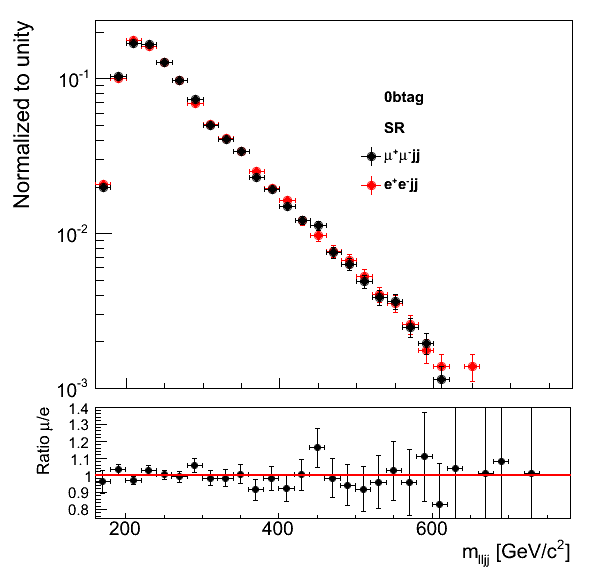
\includegraphics[width=0.33\textwidth]{plots/mH_lim20_0btag_NORM_LOG.png}
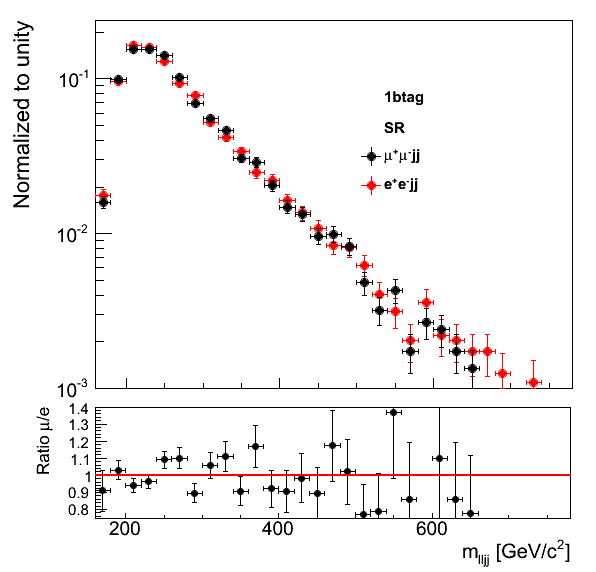
\includegraphics[width=0.33\textwidth]{plots/mH_lim20_1btag_NORM_LOG.png}
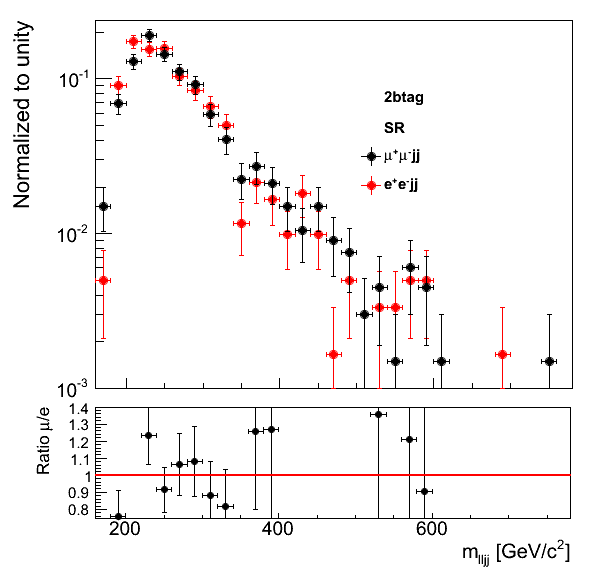
\includegraphics[width=0.33\textwidth]{plots/mH_lim20_2btag_NORM_LOG.png}
}
\centerline{
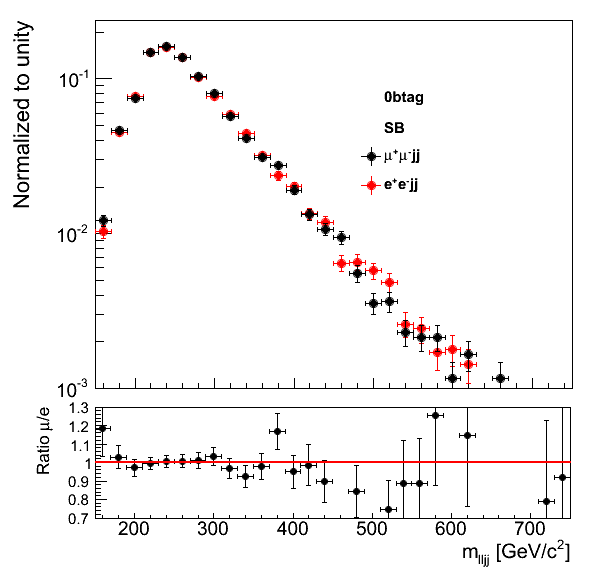
\includegraphics[width=0.33\textwidth]{plots/mH_lim20_0btag-SB_NORM_LOG.png}
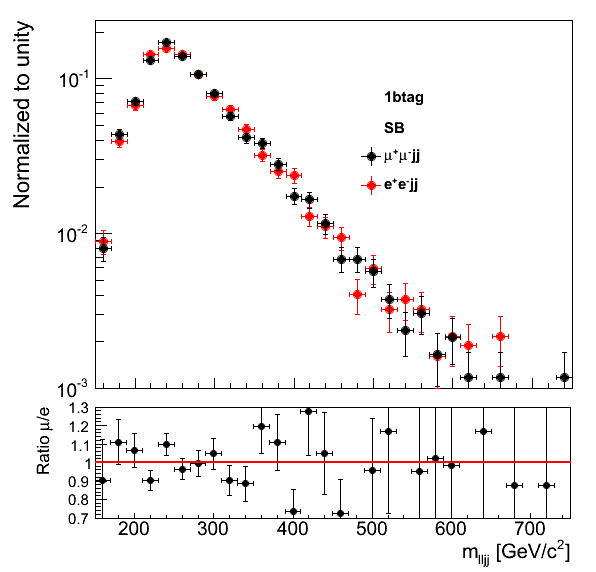
\includegraphics[width=0.33\textwidth]{plots/mH_lim20_1btag-SB_NORM_LOG.png}
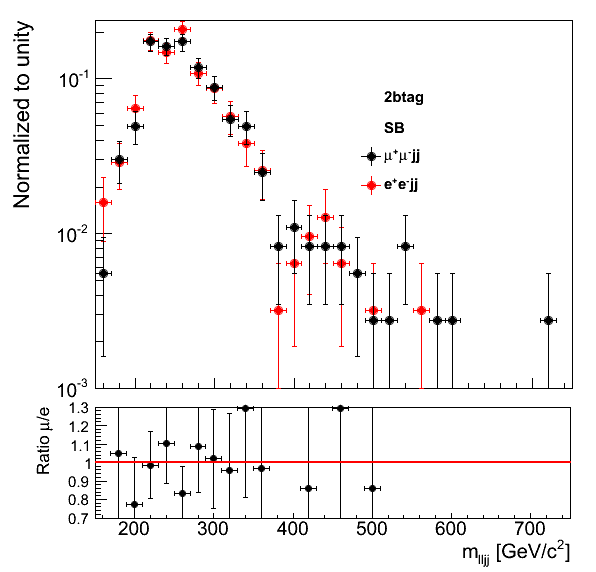
\includegraphics[width=0.33\textwidth]{plots/mH_lim20_2btag-SB_NORM_LOG.png}
}
\caption{Mass distributions of the $\LL jj$ system for events in the
electron and muon channels: data in the $m_{jj}$
(top) signal and (bottom) sideband regions.
From left to right, plots
correspond to the 0-, 1-, and 2-btag categories.
}
\label{fig:emuratios}
\end{center}
\end{figure}

